% This must be in the first 5 lines to tell arXiv to use pdfLaTeX, which is strongly recommended.
\pdfoutput=1

\documentclass[11pt]{article}

% Standard package includes
\usepackage[review]{ACL2023}
% \usepackage{ACL2023}
\usepackage{times}
\usepackage{latexsym}
\usepackage[T1]{fontenc}
\usepackage[utf8]{inputenc}
\usepackage{microtype}
\usepackage{inconsolata}
\usepackage{graphicx}
\usepackage{caption}

\setlength\titlebox{5cm}

\title{Instructions for ACL 2023 Proceedings}

\author{Zhanna Klimanova \\
  Department of Engineering \\
  University of McGill \\
  Montreal, Canada \\
  \texttt{zhanna.klimanova@mcgill.ca} \\\And
  Person 2 \\
  Department of  \\
  University of McGill \\
  Montreal, Canada \\
  \texttt{@} \\\And
  Person 3 \\
  Department of \\
  University of McGill \\
  Montreal, Canada \\
  \texttt{@} \\}

\begin{document}
\maketitle

\begin{abstract}
% Abstract: A short overview of the paper.

This paper investigates the Text-to-SQL task, which translates natural language queries (NLQ) into SQL, has broad applications: it enables non-technical users to access databases, improves customer support efficiency, and aids developers in crafting precise SQL queries. Advances in pre-trained large language models (LLMs) have shown promise in managing the complexities of natural language understanding and SQL generation. Text-to-SQL could streamline interactions on database-driven websites by replacing input fields with direct language-based querying, especially when SQL is needed for data retrieval.
[ZHANNA]

**This abstract is a good introduction but should also summarize methods and findings (can finish this after the other sections)
\end{abstract}

\section{Introduction}

% Introduction: What is the motivation behind the project? In general terms, what is the
% hypothesis that you test and how do you go about doing so?

Text-to-SQL is a critical area of research focused on the automatic translation of natural language questions into SQL queries. By bridging the gap between non-expert users and database systems, it significantly enhances data accessibility, streamlines data processing, and enables applications such as intelligent database services, automated data analysis, and database-driven question-answering systems. In this project, we evaluate the capabilities of large language models (LLMs) on a novel domain: the Cantus Database, a rich collection of metadata from Latin chants in manuscripts and early printed books, accessible at https://cantusdatabase.org.

Cantus Database is a website and database of Latin ecclesiastical chants from manuscripts and other sources around the world. It is actively maintained by developers at McGill University and is used by more than 250 academics and researchers. In the Cantus Database, there are three main objects that are searchable and filterable on the site: Chants, Sources, and Feasts. Chants are individual pieces of liturgical music, often drawn from Gregorian chant traditions, that include musical notation, text, and associated metadata. Sources refer to manuscripts or early printed books that preserve these chants, providing critical historical context for their transmission and use. Feasts are specific liturgical celebrations within the Christian calendar, such as Christmas or Easter, to which chants are assigned and performed.

The Cantus Database is structured to provide a simple yet effective way for researchers to locate specific data for their projects. However, the current search and filtering options are limited to the predefined criteria available on the site, which can restrict users who need to perform more specialized queries. To address this, we offer a solution that allows users to search the database using natural language questions (NLQs). By allowing users to input queries in their own words, the system can retrieve relevant results without being constrained by existing filters, providing greater flexibility and precision in accessing the desired information.


Specifically, the research explores whether modern pre-trained LLMs, OpenAI’s o1, xAI’s Grok, and Anthropic’s Claude, can address complex Text-to-SQL problems within the Cantus database schema without explicit fine-tuning or task-specific training. By relying solely on inference, this experiment investigates the extent to which the learned parameters of these models enable Text-to-SQL functionality, using only a natural language query, a database schema, and select schema content as inputs.


This evaluation focuses on simple prompting with GPT, Grok, and Claude on a dataset that has never been tested for Text-to-SQL tasks before. By using only natural language queries, the database schema, and select schema content as inputs, we aim to determine whether inference alone can effectively generate SQL queries without fine-tuning.

We explore GPT, Grok, and Claude to address practical limitations. Training new models has a significant environmental impact due to high computational costs. Additionally, in real-world settings, changes to the database structure often require fine-tuning or retraining, which is time-consuming and resource-intensive. To overcome these challenges, we use inference-based evaluation, as the Cantus database lacks a sufficiently large annotated dataset of Text-to-SQL data. This approach reduces costs and avoids retraining, offering a more efficient and sustainable solution.
\section{Related Work}

% Related work: Summarize previous work in the area that you have found. I don't expect you to give a complete and fully up-to-date survey of related work in the area. Instead, aim to cite and discuss at least 3-5 relevant papers, with a focus on how your work differs from theirs.

Generating SQL queries from natural language has become a critical task in natural language processing, driven by the capabilities of large language models (LLMs) to capture complex patterns within a provided database schema. The work presented in this paper shares similarities with an older study from 2022 conducted in \cite{rajkumar2022texttosql}, which highlighted that scaling training data and model size in generative language models enables advanced functionalities, such as few-shot learning without the need for task-specific finetuning. Notably, the work in \cite{rajkumar2022texttosql} demonstrates that models like Codex and GPT-3 serve as competitive Text-to-SQL solutions even without additional finetuning, a finding that aligns with this study's use of OpenAI's newer models for similar purposes. However, there are key differences. Unlike this paper, which evaluates a consistent natural language query prompt across varied data types, the work in \cite{rajkumar2022texttosql} explores varied prompts and benchmarks the performance of models of different sizes, including Codex and GPT-3, on established datasets like Spider for cross-domain Text-to-SQL tasks. While this paper introduces and evaluates a novel dataset created specifically for this project, \cite{rajkumar2022texttosql} conducted experiments in few-shot settings using benchmarks such as GeoQuery and Scholar. These differences underscore the complementary nature of the two studies in advancing the evaluation of LLMs for Text-to-SQL tasks.

Recent work by \cite{gao2023text2sql} investigates various prompt engineering strategies for open-source large language models (LLMs) in Text-to-SQL tasks. Their study systematically evaluates prompt engineering techniques, including question representation, in-context learning, and supervised fine-tuning, on benchmark datasets such as Spider and Spider-Realistic. They propose a novel solution, DAIL-SQL, which leverages these strategies to enhance the effectiveness and efficiency of Text-to-SQL performance. Unlike \cite{gao2023text2sql}, this project focuses on evaluating LLMs on a smaller, custom-built dataset derived from the Cantus Database. The primary aim is to explore how pre-trained LLMs identify patterns in the data without relying on supervised fine-tuning, keeping the data and prompts consistent. While both studies emphasize prompt engineering, they differ in scope and methodology. \cite{gao2023text2sql} provides an extensive empirical analysis of prompt engineering strategies, including zero-shot scenarios, example selection, and organization strategies in few-shot learning. Their research also highlights the potential of open-source LLMs in both in-context learning and supervised fine-tuning. In contrast, this study utilizes primarily closed-source, proprietary LLMs, focusing on their pre-trained capabilities. Like \cite{gao2023text2sql}, this study manually tested several prompt engineering methods before selecting and standardizing those used in the data.json files. However, the goal in \cite{gao2023text2sql} is to compare the performance of various LLMs rather than systematically optimizing prompt engineering strategies.

The most recent work by \cite{zetterman2024text2sql}, conducted in 2024, explores alternatives to OpenAI's GPT-3.5 and GPT-4 for Text-to-SQL tasks. This research compares Claude Opus, an advanced proprietary LLM, with a fine-tuned Mixtral 8x7B, an open-source model. Both models are evaluated on the BIRT dataset using execution accuracy as the primary metric, which involves comparing the resulting rows from executed SQL queries against ground-truth outputs. This approach provides a practical measure of model performance by assessing how well the generated SQL captures the intended query semantics. Zetterman’s work shares similarities with this study in its emphasis on evaluating the quality of generated SQL by comparing the output data to golden standards. However, while Zetterman utilizes the BIRT benchmark dataset, this project evaluates models on a smaller, custom-built dataset derived from the Cantus Database, which focuses on historical and musicological data. Additionally, Zetterman employs fine-tuning on smaller LLMs, such as Mixtral, to enhance domain-specific performance, whereas this study relies exclusively on pre-trained capabilities of both open and closed-source LLMs without performing any fine-tuning. Furthermore, Zetterman’s thesis investigates the practical trade-offs between proprietary and open-source models, emphasizing resource efficiency and accessibility. In contrast, this study prioritizes the robustness of pre-trained models when exposed to promp-engineering techniques, particularly focusing on the pre-trained model's ability to quickly find pattern in the domain-specific dataset. While both works assess execution accuracy, Zetterman’s focus on large-scale, standardized datasets contrasts with this study’s exploration of a niche, highly specialized dataset to understand LLM behavior in specific contexts.


In conclusion, while the works by \cite{rajkumar2022texttosql}, \cite{gao2023text2sql}, and \cite{zetterman2024text2sql} offer valuable insights into the capabilities of large language models (LLMs) for Text-to-SQL tasks, they each operate in contexts distinct from this study. None of these works explore Grok, the specific LLM employed in this project, which represents a novel angle of investigation. Additionally, these studies focus on established datasets like Spider, GeoQuery, Scholar, and BIRT, which are significantly larger and have likely been exposed to LLMs during pretraining or finetuning stages. In contrast, this study introduces a custom-made dataset derived from the Cantus Database, which is specialized, domain-specific, and previously unused in the training, pretraining, or finetuning of LLMs. By relying solely on prompt engineering to evaluate pre-trained LLMs, this work avoids finetuning or supervised learning, focusing instead on leveraging the models' inherent capabilities for inference. This approach not only highlights the adaptability of LLMs to unique datasets but also emphasizes the potential of prompt engineering as a lightweight yet effective strategy for extracting meaningful performance in domain-specific Text-to-SQL tasks.

PROOFREAD AND IMPROVE (LUCAS, CHARLES, ZHANNA)
\section{Methodology}
Our methodology is summarized in the workflow illustrated in \textit{Figure~\ref{fig:methods-overview}}.

\begin{figure}[h!]
    \centering
    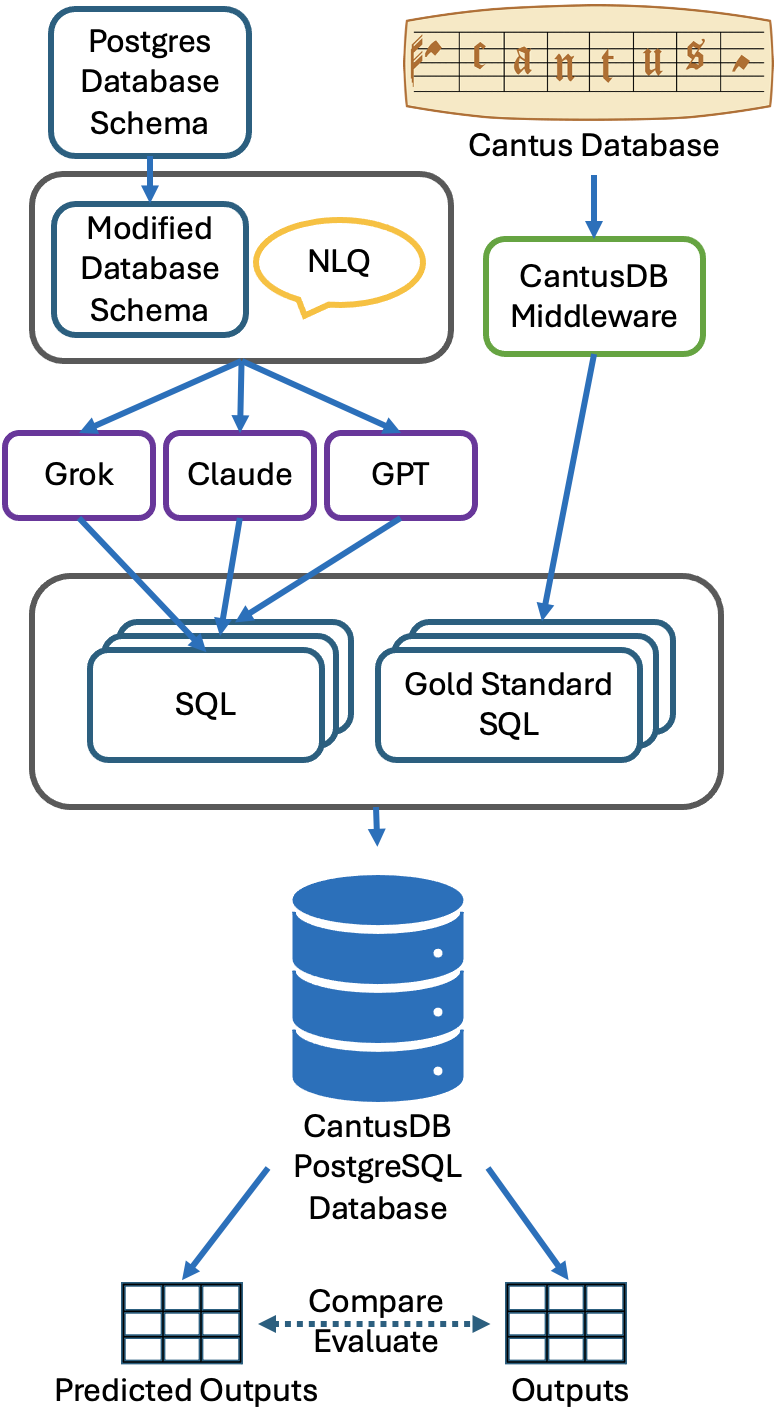
\includegraphics[width=0.35\textwidth]{Figures/methods-workflow.png} % Adjust width as needed
    \caption{Overview of the methodology: Ground truth SQL queries from Cantus Database and natural language queries with a database schema are used to prompt LLMs. The generated SQL queries are executed on the PostgreSQL Cantus Database, and the resulting object IDs are compared and evaluated.}
    \label{fig:methods-overview} % Label for referencing the figure
\end{figure}

\subsection{Overview}
Ground truth data is collected from Cantus Database using a locally deployed version of the website\footnote{Setup instructions are available at \url{https://github.com/DDMAL/CantusDB/wiki}.}. To capture SQL queries made on the database, a custom middleware is integrated into the codebase\footnote{Middleware setup instructions are detailed in the project’s README.md file.}. Additionally, a PostgreSQL database dump is used to extract the database schema. To fit within the context token limits of modern LLMs, the schema is reduced in size and complexity. The details of the reduction process are provided in Section \ref{sec:prompt_engineering}.

Ground truth and predicted data are stored in JSON files, organized by LLM (GPT, Claude, Grok) and object type (\textit{Chants}, \textit{Feasts}, and \textit{Sources}). Each entry includes the gold SQL query, output path, and natural language input. LLMs are prompted with the database schema and queries to generate SQL, which is executed in a PostgreSQL Docker container to produce CSV outputs. Paths to these outputs are recorded alongside the ground truth.

\subsection{Dataset}
The dataset consists of 45 ground truth samples, with 15 samples for each object type (\textit{Chants}, \textit{Feasts}, and \textit{Sources}). Each of the three LLMs generates predictions for 15 natural language input samples per object type, producing a total of 45 predicted SQL queries and corresponding outputs per schema. For both schema variations (with and without options) and all three object types, this totals 135 predicted outputs per schema and 270 combined. This structured approach enables a thorough evaluation of the LLMs' performance across different schema complexities and object types.

\subsection{Prompting Large Language Models}
To generate SQL queries using the LLMs, we create prompts that integrate the modified database schema with natural language inputs. To clearly differentiate values and attributes from regular text, we enclose values in single quotes and capitalize attribute names. An example of such a prompt is:
\begin{quote}
\textit{``Given this database schema, generate a SQL query that shows me all the Sources in the `CANTUS Database' Segment as a Complete Source, from the Country `Germany' and Provenance `Aachen', sorted by institution siglum and source shelfmark. Format your response without any formatting or newlines.''}
\end{quote}

Once the natural language inputs and schemas are finalized, they are provided as prompts to the GPT, Claude, and Grok models. Each LLM generates an SQL query in response to the given prompts. These queries are executed on the PostgreSQL database on CantusDB, producing outputs that include lists of IDs corresponding to the search results for \textit{Chants}, \textit{Sources}, or \textit{Feasts}—objects aligned with the search pages on Cantus Database website. The generated outputs are compared to the ground truth results, i.e., the SQL query outputs obtained directly from the PostgreSQL database. The evaluation methodology, detailed in Section \ref{sec:evaluation_metrics}, combines various techniques to assess the accuracy and usability of the SQL queries generated by the LLMs within the context of Cantus Database.

\subsection{Prompt Engineering}
\label{sec:prompt_engineering}
The LLMs are provided with a modified database schema and a natural language input as context. The schema is generated by systematically processing the PostgreSQL database dump through the following steps:

\begin{enumerate}
    \item Extract the database schema using PostgreSQL's schema-only dump feature.
    \item Filter out only the table creation statements from the schema dump.
    \item Include essential constraints, such as primary keys, foreign keys, and references.
    \item Simplify the schema by removing non-essential modifiers, such as deferrable constraints.
    \item Clean up leading whitespace and other formatting inconsistencies.
    \item Integrate the fixed values into the database schema to produce the extended version.
\end{enumerate}

In the sixth step, we introduce an extended version (with options) of the database schema that includes fixed values relevant for filtering data on Cantus Database website but absent in the raw schema. This extended schema aims to evaluate whether adding such contextual details improves the performance of SQL queries generated by the LLMs. The fixed values are outlined below.
\begin{itemize}
    \item External identifiers for standard metadata repositories: RISM Online, VIAF, Wikidata, GND, Biblioth\`{e}que Nationale de France, Library of Congress, and DIAMM.
    \item Source completeness statuses: Full Source, Fragment, Reconstruction, and Fragmented.
    \item Temporale and Sanctorale prefixes used for Feast filtering.
    \item Proofreading status: Any, Yes, or No.
\end{itemize}

\subsection{Evaluation Metrics}
\label{sec:evaluation_metrics}
Five quantitative evaluation metrics were used to gauge the performance of the different LLMs. The first verified if the SQL queries generated by the LLMs returned the correct elements, ignoring the order. The second metric was the ordered metric, which made sure the items were in the correct order. This was done since Cantus Database search requires the user to specify an order of the items, and this order was reflected in the natural language query. These two metrics were treated as raw counts, so a value of 32 means that 32 out of the 45 queries were correct. Since there are 45 queries in total, both metrics are out of 45.

Precision, recall, and F1 were used to assess the performance. Precision measures how many items the LLM generates are correct, reflecting how well the model avoids generating irrelevant items. Whereas recall evaluates how many correct items from the gold standard were generated by the model, indicating its ability to capture all relevant results. To balance precision and recall, the F1 score was also calculated. The F1 score is the harmonic mean of precision and recall, providing a single metric for correctness and completeness. This is particularly relevant to Cantus Database users, as maximizing precision ensures all results are accurate with no false positives, while high recall guarantees that no relevant items are omitted from the search. The final metric used is the average across the 45 queries.

\section{Results}
We evaluated the performance of three LLMs (GPT-o1, Claude, and Grok) in generating accurate SQL queries for the Cantus Database, comparing two scenarios: with and without a schema's predefined options. Results are reported as counts out of 45 for correct values with and without ordering, along with precision, recall, and F1 scores. Findings are shown in \textit{Table \ref{tab:schema_without_data}} and \textit{Table \ref{tab:schema_with_data}}.

\begin{table}[ht]
\centering
\begin{tabular}{lccc}
\hline
\textbf{Metric}             & \textbf{GPT} & \textbf{Claude} & \textbf{Grok}   \\
\hline
Unordered (count)                 & \textbf{23}  & \textbf{23}     & 16              \\
Ordered (count)                      & \textbf{16}  & 15              & 11              \\
Precision                   & 0.70        & \textbf{0.75}          & 0.56  \\
Recall                      & 0.69        & \textbf{0.74}  & 0.47           \\
F1                          & 0.68 &    \textbf{0.70}      & 0.48           \\
\hline
\end{tabular}
\caption{Results for the schema without options. The unordered and ordered metrics display counts out of 45.}
\label{tab:schema_without_data}
\end{table}

\begin{table}[ht]
\centering
\begin{tabular}{lccc}
\hline
\textbf{Metric}             & \textbf{GPT} & \textbf{Claude} & \textbf{Grok}   \\
\hline
Unordered (count)                     & \textbf{32}  & 28              & 23              \\
Ordered (count)                     & \textbf{23}  & 16              & 10              \\
Precision                   & \textbf{0.92}       & 0.85          & 0.69  \\
Recall                      & \textbf{0.88} & 0.78          & 0.60           \\
F1                          & \textbf{0.88} & 0.78          & 0.61           \\
\hline
\end{tabular}
\caption{Results for the schema with options. The unordered and ordered metrics display counts out of 45.}
\label{tab:schema_with_data}
\end{table}
\section{Discussion}

\subsection{Performance on Schema Without Options}
For schemas without options (\textit{Table \ref{tab:schema_without_data}}), GPT and Claude achieve the highest unordered scores, each with 23 correct queries out of 45, while Grok trails with 16. For ordered results, GPT leads with 16 correct queries, followed by Claude with 15, and Grok with 11.

Precision, recall, and F1 scores provide a better understanding of the models' performance. While GPT and Claude generate the same number of correct unordered queries, Claude outperforms GPT in overall metrics, achieving a precision of 0.75, a recall of 0.74, and an F1 score of 0.70. This suggests that Claude's incorrect queries are generally closer to being correct. GPT follows closely with a precision of 0.70, a recall of 0.69, and an F1 score of 0.68. Grok lags behind both, with a precision of 0.56, a recall of 0.47, and an F1 score of 0.48.

\subsection{Performance on Schema with Options}
All models demonstrate improved performance when schemas include options (\textit{Table \ref{tab:schema_with_data}}). GPT leads with the highest unordered count of 32 and ordered count of 23, followed by Claude with unordered and ordered counts of 28 and 16, respectively. Grok shows the weakest performance, with unordered and ordered counts of 23 and 10, respectively.

All models also show improved precision, recall, and F1 scores when provided with schema options. GPT achieved the most significant gains, leading with scores of 0.92 for precision and 0.88 for both recall and F1. Claude also improved, though less markedly, with scores of 0.85 for precision and 0.78 for recall and F1. Grok, while showing some progress, remained the weakest performer, with precision at 0.69, recall at 0.60, and F1 at 0.61.

\subsection{Implications and Insights}
The results indicate that GPT achieves the best outcomes when schema options are available, demonstrating its ability to leverage additional information to enhance performance. In contrast, Claude delivers stronger results without schema options, suggesting strength in handling more ambiguous contexts. Lastly, Grok consistently lags behind under both conditions.

\subsection{Limitations}
One limitation of this research is that the CantusDB user interface limits the kinds of queries that can be generated. Addressing this presents an interesting opportunity for future research. However, it would require more effort, as the SQL queries would need to be written manually instead of generated automatically by the website.

Another limitation is the reliance on metrics that evaluate query result matching rather than SQL correctness, potentially overlooking syntax validity, query complexity, and edge cases. Adding contextual relevance metrics could better assess how well generated queries reflect the intent of the natural language input, considering ambiguity and phrasing.

The methodology could also be improved with greater automation. Manual updates to data files and results are prone to errors and labor-intensive. Automating this process with scripts would minimize errors and enable future iterations to handle larger datasets efficiently.

Lastly, extraneous information adds noise and hinders performance, while missing details force models to make assumptions, leading to incorrect queries. Providing specific values in the prompt ensures the generated SQL queries align with the database. Future research is needed to refine the schema structure to optimize performance and better reflect user-based natural language queries.
\section{Conclusion}

This research confirmed the hypothesis that large language models can generate SQL queries for the specialized Cantus Database without fine-tuning. GPT achieved the best performance with schema options, correctly generating 32 out of 45 queries (ignoring order) and reaching an F1 score of 0.88. In the absence of options, Claude outperformed the other models, generating 23 correct queries and achieving an F1 score of 0.70. Grok consistently performed the weakest in both scenarios. The study underscores that incorporating select schema values with natural language queries significantly enhances performance across all models, demonstrating that modern large language models can address domain-specific Text-to-SQL tasks through prompt engineering alone. This efficient approach provides a viable alternative to fine-tuning, and future work could explore broader query types beyond the current limitations of Cantus Database.

\section{Contributions}

The project was a collaborative effort, with Zhanna leading the project setup, literature review, and JSON design. Lucas and Charles focused on schema generation and middleware, with Lucas also assisting with the Cantus Database setup and data extraction pipeline. Data generation was divided, with Zhanna handling GPT, Charles working with Grok, and Lucas managing Claude. Evaluation metrics were discussed by all, with Charles leading the analysis. Zhanna set up the LaTeX document and started the report, with all members contributing to every section. Regular meetings ensured clear tasks, progress, and revisions, highlighting strong teamwork.
\appendix

\section{Example Appendix}
\label{sec:appendix}

This is a section in the appendix.


\bibliography{references}
\bibliographystyle{acl_natbib}

\end{document}
